%-------------------------------------------------------------------------------
%-------------------------------------------------------------------------------
\section{Discussion}
%-------------------------------------------------------------------------------
%-------------------------------------------------------------------------------

%==================================================================
\frame{\frametitle{Network inference}

  \paragraph{Network inference is} 
  \begin{itemize}
   \item Not always a very well-posed problem
   \item A difficult task because of its combinatorial dimension ('a needle in a haystack')
   \item Slightly easier for undirected networks
   \item A highly unsupervised problem (nobody knows the truth, few experimental validations exist)
  \end{itemize}
  
  \bigskip \bigskip \pause
  \begin{tabular}{ll}
    \hspace{-.04\textwidth}
    \begin{tabular}{p{.6\textwidth}}
      \paragraph{Take-home-message} 
      \begin{itemize}
      \item It is not hopeless (although ...)
      \item Graphical models provide a sound mathematical framework 
      \item Reasonably simple tools (R packages) exist 
      \item Accounting for samplign effort and covariates has a dramatic effect on the inferred network
      \item Always ask if the question is a network question \refer{JFS16}
      \end{itemize}
    \end{tabular}
    &
    \pause
    \hspace{-.05\textwidth}
    \begin{tabular}{p{.4\textwidth}}
      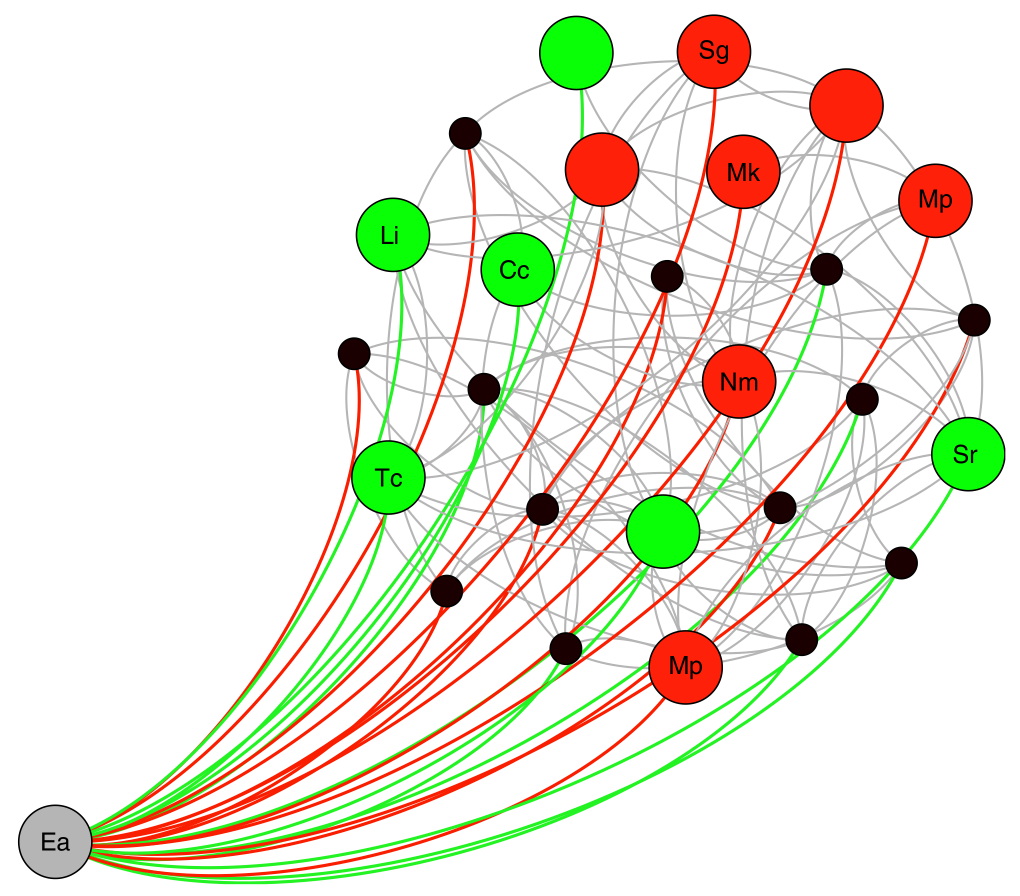
\includegraphics[width=.3\textwidth]{\fignet/JFS16-EnvirMicrobiol-Fig4}
    \end{tabular}
  \end{tabular}

}

%==================================================================
\frame{\frametitle{Network structure}
  
  \paragraph{Statistical models = random graph models.} Can be used to \\~
  \begin{itemize}
    \item exhibit latent structure \\~
    \item correct for expected effects (e.g. covariates) and enhanced unexpected ones
%     \item to serve as (not too) null model to be compared with observation (and to exhibit some {\sl residual} structure)
  \end{itemize}

  \bigskip \bigskip \pause
  \paragraph{Many other ways to analyse a network structure (topology).} \\~
  \begin{itemize}
    \item Global descriptors: density, connectivity, 'nestedness' \\~
    \item Node characteristics: degree distribution, 'edge-betweenness'\\~
    \item Meso-scale descriptors: motifs \\~
  \end{itemize}
  \ra Again: need for a ('null') model to assess the significance of observed values (e.g; configuration model, expected degree model, etc)
    
}
